\newpage
\section{Билет 20. Отношение причинно-следственной зависимости. Метки Лэмпорта, векторные часы.}\label{b20}
\begin{center}
    \textit{\underline{Отношение причинно-следственной зависимости.}}
\end{center}
 Отношение причинно-следственной зависимости\footnote{Подробнее см. 66 с. книги «Ж. Тель. Введение в распределенные алгоритмы. М.: МЦНМО, 2009. — 616 с. — ISBN 978-5-94057-515-3.»} - это аналог понятия  «Справедливости». Можно сравнивать события и узнавать, какое из них произошло раньше, а какое позже. \\ 
Пусть в предположении у нас задано следующее:
\begin{itemize}
\item Сравнимы события в одном процессе (например, с помощью локального счётчика).
\item Сравнимы отправка и получение сообщений. (Отправка сообщения логически предшествует получению этого же самого сообщения.)
\end{itemize}
%Представляя выполнение в виде последовательности переходов, мы тем самым естественно привносим в модель понятие времени. Будем говорить, что переход $a$ происходит раньше, чем переход $b$, если в последовательности переходов событие $a$ предшествует событию $b$.\\
Хотим реализовать механизм сравнения двух событий в случае, если они сравнимы.\footnote{Узнать что произошло раньше, а что позже (транзитивное замыкание описанных двух отношений).}

Пусть $n$ - количество процессов. $\forall p = 1, \ldots, n$ заводим свой счётчик $L_p := 0;$ событий.\\
Внутри процесса могут происходить локальные события, которые мы хотим учесть при общем сравнении, поэтому мы их тоже будем помечать. (см. \nameref{algComparison})

\begin{algorithm}
\caption{Алгоритм сравнения событий. Метки Лэмпорта}
\label{algComparison}
\begin{algorithmic}
\State $L_p \gets 0$
\Function{matching}{$e$}\Comment{Приписываем событию $e$ временную метку $L(e)$ (Leslie Lamport).}
%\State 
\If{$e$ - локальное событие в процессе $p$}
    \State $L_p += 1$
    \State $L(e) \gets L_p$ \Comment{Нумеруем локальное событие своим же счётчиком.}
\EndIf
\If{$e$ - отправка сообщения $message$ процессу $q$ от процесса $p$}
    \State $L_p += 1$
    \State $send(<message, L_p>, q)$ \Comment{Вместе с данными передаём свою метку времени.}
\EndIf
\If{$e$ - получение сообщения $<message, L>$ от процесса $q$ в  процессе $p$}
    \State $L_p \gets \max\{L,L_p\} + 1$
    \State $L(e) \gets L_p$ \Comment{Получение сообщения тоже может быть учтено как событие $e$.}
\EndIf
\EndFunction
\end{algorithmic}
\end{algorithm}

%Приписываем событию $e$ временную метку $L(e)$ (Leslie Lamport).\\ \\
%Когда происходит локальное событие $e$ в процессе с номером $p$:\\
%\ \ \ \ $L_p += 1;$\\
%\ \ \ \ $L(e) = L_p;$ //Нумеруем локальное событие своим же счётчиком. \\ \\ 
%Отправка сообщения $message$ процессу с номером $q$ от процесса с номером $p$:\\
%\ \ \ \ $L_p += 1;$\\
%\ \ \ \ $send(<message, L_p>, q);$ //Вместе с передаваемыми данными передаём свою метку времени.\\ \\
%Получение сообщения $<message, L>$ от процесса с номером $q$ в  процессе с номером $p$:\\ 
%\ \ \ \ $L_p = \max\{L,L_p\} + 1;$\\
%\ \ \ \ $L(e) = L_p;$ //Получение сообщения тоже может быть учтено как событие $e$. \\

\textbf{Итого:} У всех исходно нулевой счётчик. Каждому событию, которое мы хотим сравнивать, приписываем числовую временную метку. Для локальных событий в $p$ увеличиваем локальный счётчик на $1$. Отправляя сообщение, локально подписываем факт отправки и затем отправляем свою метку. Получая сообщение, вычисляем максимум временных меток.

Пусть событие $e_1$ произошло точно раньше события $e_2$ по нашему заданному отношению причинно-следственной зависимости (либо произошли в одном процессе и $e_1$ раньше $e_2$, либо в разных, но между ними $\exists$ цепочка попарно-сравнимых событий).
Тогда $L(e_1) < L(e_2)$. (По построению будет так)

\textbf{Замечание:} Обратное неверно! (См. рисунок. \ref{fig:Image_comparsion})

\begin{figure}[H]
\center{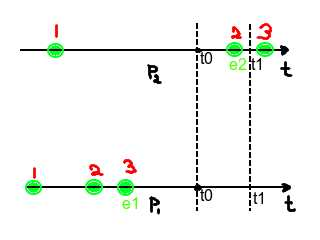
\includegraphics[width=0.9\textwidth]{20/Comparison_for_labels.jpg}}
\caption{В момент $t_0$: $2 = L_{p_2} < L_{p_1} = 3$, хотя событие $e_1 < e_2$.} 
\label{fig:Image_comparsion}
\end{figure}
        
Для выполнения необходимого и достаточного условия ($e_1 < e_2 \Leftrightarrow L(e_1) < L(e_2)$) реализуют механизм под названием «векторные часы». Разница с предыдущим алгоритмом лишь в том, что во всех процессах ведётся учёт временных меток не одного процесса, а целого вектора (массива) временных меток $\bar{L}_p := (L_p^1, \ldots, L_p^n)^T$ всех процессов.
Приведём \nameref{algComparisonVecClock}.
\begin{algorithm}
\caption{Алгоритм сравнения событий. Векторные часы}
\label{algComparisonVecClock}
\begin{algorithmic}
\State $L_p \gets (\underbrace{0,\ldots,0}_{n}) = \bar{0}$
\Function{matching}{$e$} \Comment{Приписываем событию $e$ временную метку $L(e)$ (Leslie Lamport).}
\If{$e$ - локальное событие в процессе $p$}
    \State $L_p[p] += 1$
    \State $L(e) \gets L_p$ \Comment{Нумеруем локальное событие своим же счётчиком.}
\EndIf
\If{$e$ - отправка сообщения $message$ процессу $q$ от процесса $p$}
    \State $L_p[p] += 1$
    \State $send(<message, L_p>, q)$ \Comment{Вместе с данными передаём свою метку времени.}
\EndIf
\If{$e$ - получение сообщения $<message, L>$ от процесса $q$ в  процессе $p$}
    \For{$i = 1, \ldots, n$}
        \State $L_p[i] \gets \max\{L[i],L_p[i]\}$
    \EndFor
    \State $L_p[p] += 1$
    \State $L(e) \gets L_p$\Comment{Получение сообщения тоже может быть учтено как событие $e$.}
\EndIf
\EndFunction
\end{algorithmic}
\end{algorithm}
%$\forall p = 1, \ldots, n$ заводим свой массив счётчиков $\bar{L}_p := \bar{0};$ событий.\\ \\
%Когда происходит локальное событие $e$ в процессе с номером $p$:\\
%\ \ \ \ $L_p[p] += 1;$\\
%\ \ \ \ $L(e) = L_p;$ //Нумеруем локальное событие своим же счётчиком. \\ \\
%Отправка сообщения $message$ процессу с номером $q$ от процесса с номером $p$:\\
%\ \ \ \ $L_p[p] += 1;$\\
%\ \ \ \ $send(<message, L_p>, q);$ //Вместе с передаваемыми данными передаём свою метку времени.\\ \\
%Получение сообщения $<message, L>$ от процесса с номером $q$ в  процессе с номером $p$:\\
%\ \ \ \ $L_p[i] = \max\{L[i],L_p[i]\};\ \forall i = 1, \ldots, n.$\\
%\ \ \ \ $L_p[p] += 1;$\\
%\ \ \ \ $L(e) = L_p;$ //Получение сообщения тоже может быть учтено как событие $e$.\\

Итого: $e_1 < e_2 \Leftrightarrow L(e_1)[i] \leq L(e_2)[i]\ \forall i = 1,\ldots, n$ покоординатно, причём $\exists i: L(e_1)[i] < L(e_2)[i]$ строго.

Если $\exists i_1, i_2 \in [1,n]: L(e_1)[i_1]< L(e_2)[i_1]$ и при этом же $L(e_1)[i_2] >  L(e_2)[i_2] $, то события $e_1$ и $e_2$ не сравнимы.

\textbf{Замечание:} Multicast, построенный на основе векторных часов - это CO-multicast. (Не можем доставить пришедшее сообщение в процесс до тех пор, пока не получили все сообщения, логически предшествующие тому, что стоит в  очереди.)
